\input{settings}
\setlength{\emergencystretch}{2em}
\titleformat{\section}
  {\small\bfseries\raggedright}
  {}{0em}
  {}
  [{\color{WHU_Blue}\titlerule}]
\titlespacing*{\section}{0cm}{0.70em}{0.45em}
\titlespacing*{\subsection}{0cm}{0.50em}{0.30em}
\setlist[itemize]{topsep=0.10em, itemsep=0.10em, parsep=0em, partopsep=0em, leftmargin=1.25em}
\setlist[enumerate]{topsep=0.10em, itemsep=0.10em, parsep=0em, partopsep=0em, leftmargin=1.35em}
\renewcommand{\arraystretch}{0.98}
\renewcommand{\CJKglue}{\hskip 0.018em}

% 个人信息
%  cd C:\Users\31087\Documents\Obsidian_Vault\Resume\template
%  xelatex main_pm.tex
\newcommand{\school}{江南大学 · 控制科学与工程}

\newcommand{\contact}{
    \scriptsize
    \textcolor{white}{
        \faEnvelope \quad \href{mailto:yuejinai55@gmail.com}{yuejinai55@gmail.com}
        \hspace{3em}
        \faPhone \quad +86 15515602693
        \hspace{3em}
        \faGithub \quad \href{https://github.com/L-yb555}{github.com/L-yb555}
    }
}

\newcommand{\resumeDecor}{
    \begin{tikzpicture}[remember picture, overlay]
        \node[anchor=north, inner sep=0pt](header) at (current page.north){
            
\includegraphics[width=\paperwidth]{images/header.png}
        };
        \node[anchor=west](school_logo) at (header.west){
            \hspace{0.5cm}
            
\includegraphics[width=0.15\textwidth]{images/whu_logo_1.png}
        };
        \node[anchor=east](school_name) at(header.east){
            \textcolor{white}{\textbf{\school}}
            \hspace{0.5cm}
        };
    \end{tikzpicture}

    \begin{tikzpicture}[remember picture, overlay]
        \node[anchor=south, inner sep=0pt](footer) at (current page.south){
            
\includegraphics[width=\paperwidth]{images/footer.png}
        };
        \node[anchor=center] at(footer.center){\contact};
    \end{tikzpicture}

    \begin{tikzpicture}[remember picture, overlay]
        \node[opacity=0.05] at(current page.center){
            
\includegraphics[width=0.68\paperwidth, keepaspectratio]{images/whu_logo_big.png}
        };
    \end{tikzpicture}
}

\newcommand{\sectionIcon}[2]{\makebox[\widthof{#1}][c]{\color{WHU_Blue}{#1}}\quad #2}

%%%%%%%%%%%%%%%%%%%%
% 简历正文
%%%%%%%%%%%%%%%%%%%%
\begin{document}
\resumeDecor
\vspace*{-3.15em}
\scriptsize
\linespread{1.11}\selectfont

% 个人信息
\begin{minipage}{0.80\textwidth}
    \section[个人信息]{\sectionIcon{\faAddressCard}{个人信息}}
    \begin{tabularx}{\linewidth}{p{\widthof{求职意向:}}Xp{\widthof{最高学历:}}X}
        姓\ \ \ \ \ \ \ \ 名: & 梁邦一 &
        性\ \ \ \ \ \ \ \ 别: & 男 \\
        年\ \ \ \ \ \ \ \ 龄: & 24岁 &
        政治面貌: & 共产党员 \\
        英语等级: & CET-6 &
        求职意向: & 项目管理岗 \\
    \end{tabularx}
\end{minipage}
\hfill
\begin{minipage}{0.12\textwidth}
    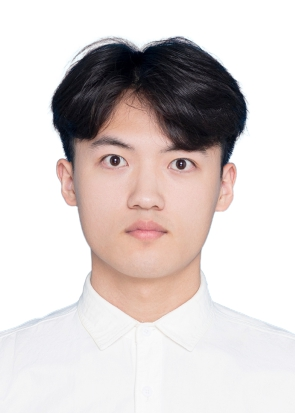
\includegraphics[width=\linewidth]{images/avatar.png}
\end{minipage}
\vspace{-1.28em}

\section[教育背景]{\sectionIcon{\faGraduationCap}{教育背景}}
\begin{itemize}
    \item {\textbf{控制科学与工程硕士，江南大学}} \hfill {2024.06--2027.06}
    \item {\textbf{自动化学士，郑州轻工业大学}} \hfill {2020.09--2024.06}
\end{itemize}

% 荣誉与组织经历
\section[荣誉与组织经历]{\sectionIcon{\faStar}{荣誉与组织经历}}
\begin{itemize}
    \item \textbf{本科班长}（2020.10--2024.06，任期 4 年）：统筹管理 60 人班级事务，对接学院老师与班级分工，策划 3 场以上大型班级活动；\textbf{硕士党支部书记}（2024.10--2026.05）：组织支部活动与成员协调，累计 6 年学生干部经历，沉淀\textbf{跨角色沟通、需求收集、任务拆解与落地推进}能力。
    \item \textbf{中国机器人大赛暨 RoboCup 机器人世界杯中国赛} 国家三等奖（本科期间，参与机器人竞赛全流程）；校一等奖学金（2025.10）；优秀毕业生（2024.06）。
\end{itemize}

% 专业技能
\section[专业技能]{\sectionIcon{\faWrench}{专业技能}}
\begin{itemize}
    \item \textbf{项目全流程管理}：需求拆解、里程碑规划、资源统筹、跨模块协同、方案评审与交付验收；具备\textbf{独立担任项目负责人}的 12 个月端到端项目推进经验，能够将业务目标拆解为可执行任务并推动方案落地。
    \item \textbf{跨部门协同与客户对接}：6 年学生干部经历，累计对接学院、班级、支部多方角色；本科期间任产品顾问，1v1 深度客户访谈、需求挖掘、定制化方案设计与沟通；实习中对接标注、算法、验收多方，具备\textbf{需求转技术方案}与推动多方达成共识的能力。
    \item \textbf{制造业与工程背景}：自动化本科背景，覆盖自动控制、电路、信号与系统、微机原理、嵌入式系统等课程；具备汽车制造一线 PLC 控制程序优化实习经验，熟悉\textbf{设备规格书解读、控制逻辑设计、生产验证}的完整交付流程。
    \item \textbf{工程与文档工具}：Python、C++、Linux/Ubuntu、Git 版本管理、ROS2、PyTorch；Markdown/LaTeX 结构化文档、Figma 界面原型、流程图与技术方案设计；熟练使用 Claude Code / Codex 等 AI 工作流工具搭建文档生成与审校 Agent，提升团队产出效率。
\end{itemize}

% 实习经历
\section[实习经历]{\sectionIcon{\faBriefcase}{实习经历}}

\vspace{0.04em}
{\normalsize\textbf{CARIZON（大众×地平线合资智驾）}}  感知数据部门算法实习生 \hfill {2026.06--至今}\\
\textbf{跨部门协同 / 数据交付验收 / 调用链梳理与团队交接支撑}
\begin{enumerate}
    \item 对接标注、算法、验收三方需求，设计红绿灯场景转向 Tagger 挖掘规则，在 3W 条路口数据中筛选 3K 条转向 CLIP，标签验收准确率达 90\%，满足业务方交付标准。
    \item 主导 1.8 万张挡轮杆候选图像的清洗、标注校验与 Prompt 迭代全链路，推动多轮验收反馈闭环，完成模型二次精标业务交付要求；另设计"规则渲染 + 生成模型"合成 pipeline，产出 5K 张 Corner Case 训练样本填补实车采集空白。
    \item 系统性梳理 mining-system 从 config.yaml、tagger 配置、推理接口到模型 worker 的调用链，建立模型版本与 checkpoint 映射关系，\textbf{支撑复杂刷库任务的问题排查与团队交接}，提升跨团队协作透明度。
\end{enumerate}

\vspace{0.04em}
{\normalsize\textbf{苏州烽奇闪盈科技有限公司}}  产品顾问 \hfill {2022.05--2022.09} \\
\textbf{客户对接 / 需求挖掘 / 定制化方案交付}
\begin{enumerate}
    \item 以 1v1 访谈形式每周与 6--8 名核心客户沟通，深入挖掘资产配置真实痛点与潜在需求，沉淀高频需求与用户痛点，为后续方案匹配提供依据。
    \item 综合客户财务状况、风险偏好等多维度信息，每周独立撰写《周度人物画像汇总报告》，提升目标客户分层、需求判断与方案推荐的准确性；累计交付 \textbf{50+ 份《产品建议书》}，清晰阐述匹配逻辑与预期价值，沉淀需求分析、方案表达与客户沟通能力。
\end{enumerate}

\vspace{0.04em}
{\normalsize\textbf{长兴和良智能制造有限公司}}  研发实习生 \hfill {2024.05--2024.09} \\
\textbf{制造业一线 / 需求转技术方案 / 生产验证闭环}
\begin{enumerate}
    \item 深度参与汽车制造流程，负责核心生产设备（汽车空调弯管机）的 PLC 控制程序优化项目，将负责人下达的性能提升目标转化为可执行技术方案，推动优化思路进入生产验证。
    \item 独立完成设备原始规格书解读与分析，运用流程图等工具梳理与设计优化后的程序逻辑，输出可用于开发沟通与方案评审的流程文档；控制程序优化方案在实际生产环境稳定运行，积累"现场需求 → 控制逻辑 → 交付验证"完整工程经验。
\end{enumerate}

\vspace{0.04em}
\section[科研与项目经历]{\sectionIcon{\faFlask}{科研与项目经历}}

\vspace{0.04em}
{\normalsize\textbf{灵心巧手 — 多模态感知与灵巧手抓取控制系统 · 项目负责人}} \hfill {2025.02--2026.02} \\
\textbf{项目全流程管理 / 资源统筹 / 跨模块协同 / 交付输出 \hfill GitHub: \href{https://github.com/L-yb555/semg-force_ui}{github.com/L-yb555/semg-force\_ui}}
\begin{enumerate}
    \item \textbf{独立牵头}人机交互多模态实验系统从 0 到 1 建设，拆解为硬件采集 → 算法训练 → 仿真验证 → ROS2 联调 → Web/VR 演示 5 大阶段，输出里程碑计划与交付清单，历时 12 个月完成端到端项目闭环。
    \item 统筹 Delsys Trigno 肌电、Sensel 压力、Linker Hand G20 灵巧手、MuJoCo 仿真环境、Linux 服务器与多机 GPU 训练资源等设备/软件资源，与导师、器材供应方沟通预算与设备到位节奏，保障各阶段实验准时启动。
    \item 设计 ROS2 Topic 分层通信接口，明确视觉、仿真策略、肌电力估计、触觉反馈四大模块的输入输出边界，使各模块\textbf{可独立替换、调试与验证}，降低团队协作与后续交接成本；完成代码仓库、运行文档、Figma 原型、技术方案与展示稿输出，成果转化为 3 篇学术论文与可演示 Web/VR 系统。
\end{enumerate}

\section[论文与研究成果]{\sectionIcon{\faBook}{论文与研究成果}}
\begin{enumerate}
    \item 已中（JCR 一区，中科院二区）：Liang B., Li N., Li G., et al. Sensing Technologies for Hand Gesture Recognition in Human-Robot Interaction: A Review[J]. IEEE Sensors Journal, 2025, 26(2): 1501-1519. 手势识别综述。
    \item 在修（JCR 一区，中科院二区 Top）：sEMG Conformer: Synergizing Local-Global Spatiotemporal Features for Continuous Force Estimation. Biomedical Signal Processing and Control.
    \item 在投（JCR 一区，中科院二区）：Dexterous Hand Grasping Control Based on Multimodal Sensory Fusion and Simulation Reinforcement Learning.
\end{enumerate}

\end{document}
